\chapter{塑料与合成材料}\label{ch:g8:plastics}

数一数，一个早上你接触到的塑料物品有多少：牙刷、
瓶子、雨衣、手机壳、公交车座椅、购物的袋子。
它们中几乎没有一样在一百二十年前已经存在，
也没有一样长在树上或是从地下挖出来的。塑料是由化学家发明的材料
——轻便、便宜、防水，可以塑造成
任何形状，而这份成功本身，如今却成了问题。

\begin{recall}
天然材料基本上按其在自然界中的原样使用；
人造材料则是由原料经加工改造而成，
而回收利用则把旧物品的材料变成新物品
（见\cref{ch:g5:raw-materials-and-recycling}）。由碳和氢组成的燃料
燃烧会生成二氧化碳和水
（见\cref{ch:g8:combustion-and-fuels}）。
\end{recall}

\begin{omfigure}
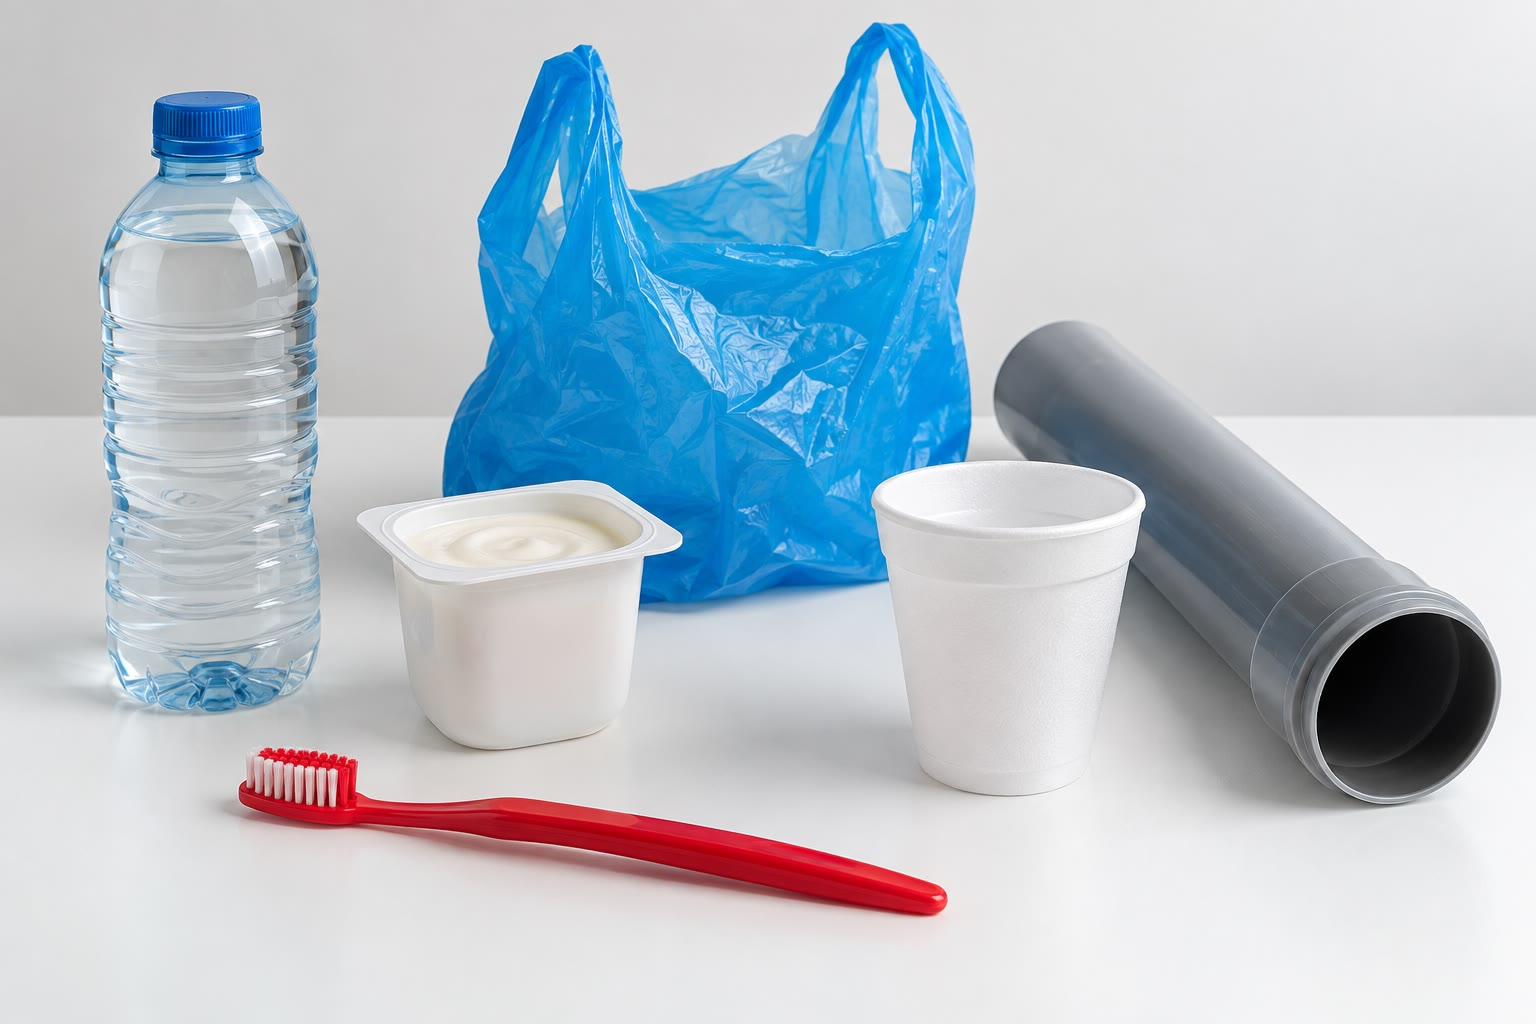
\includegraphics[width=0.55\linewidth]{images/book1/ai/g8-plastic-objects.jpg}

{\small 日常塑料物品：瓶子、盆、袋子、管子、杯子、
牙刷。}
\end{omfigure}

\section{天然材料、人造材料与合成材料}

\begin{definition}[人造材料与合成材料]\label{def:g8:plastics:artificial}
在人造材料中，通过化学方法改造天然材料而制成的，
称为\emph{人造材料}\index{人造材料}。例如，由木材纤维素制成的纸和
粘胶纤维（一种织物）。
而\emph{合成材料}\index{合成材料}是由化学家合成的物质制成，
通常以原油为原料，且没有天然的对应物：
尼龙、涤纶和塑料。
\end{definition}

\begin{omfigure}
\begin{tikzpicture}[font=\small, level distance=1.5cm,
    box/.style={draw=omDef, fill=omDef!6, rounded corners=2pt, align=center,
      inner sep=4pt, text width=3.3cm},
    level 1/.style={sibling distance=6.4cm},
    level 2/.style={sibling distance=3.8cm},
    edge from parent/.style={draw, thick, omDef, ->}]
  \node[box] {材料}
    child {node[box] {天然 \\ \footnotesize 棉、羊毛、木材}}
    child {node[box] {人造材料}
      child {node[box] {人造材料 \\ \footnotesize 纸、粘胶纤维}}
      child {node[box, draw=omProp, fill=omProp!6] {合成材料 \\ \footnotesize 尼龙、
        涤纶、塑料}}};
\end{tikzpicture}

{\small 天然材料、人造材料与合成材料。}
\end{omfigure}

\section{什么是塑料}

\begin{definition}[塑料]\label{def:g8:plastics:plastic}
\emph{塑料}\index{塑料}是一种由很长的分子构成的合成材料，
可以通过模塑加工成型——通常是在受热变软时——
并在冷却后保持形状。大多数塑料
由原油或天然气制成。
\end{definition}

\begin{remark}[很长的分子]\label{rem:g8:plastics:long}
一个水分子含有三个原子，而一个塑料分子可以含有
数万个原子，它们连成一条长链，就像一串相同的
珠子组成的项链。这种长链如何构成，
是本书末尾一章的主题。
\end{remark}

\begin{omfigure}
\begin{tikzpicture}[font=\small]
  \foreach \k in {0,...,17} {
    \pgfmathsetmacro\x{0.62*\k}
    \pgfmathsetmacro\y{0.35*sin(40*\k)}
    \shade[ball color=omDef!50] (\x,\y) circle (0.22);
  }
  \node[anchor=west] at (11.2,0) {\dots};
  \node[anchor=north, align=center] at (5.3,-0.6) {由数千个相同单元构成的长链};
\end{tikzpicture}

{\small 这是示意图而非模型：塑料分子是一条很长的
由相同单元构成的链。}
\end{omfigure}

\begin{history}[电木，1907 年]
第一种完全合成的塑料由化学家利奥·贝克兰
于 1907 年以煤焦油中提取的苯酚和甲醛为原料制成。电木坚硬、
颜色深暗、耐热，成为电话、收音机和
电器开关的材料。尼龙于 20 世纪 30 年代问世，
第二次世界大战后，瓶子和袋子所用的塑料也相继出现。
\end{history}

\begin{omfigure}
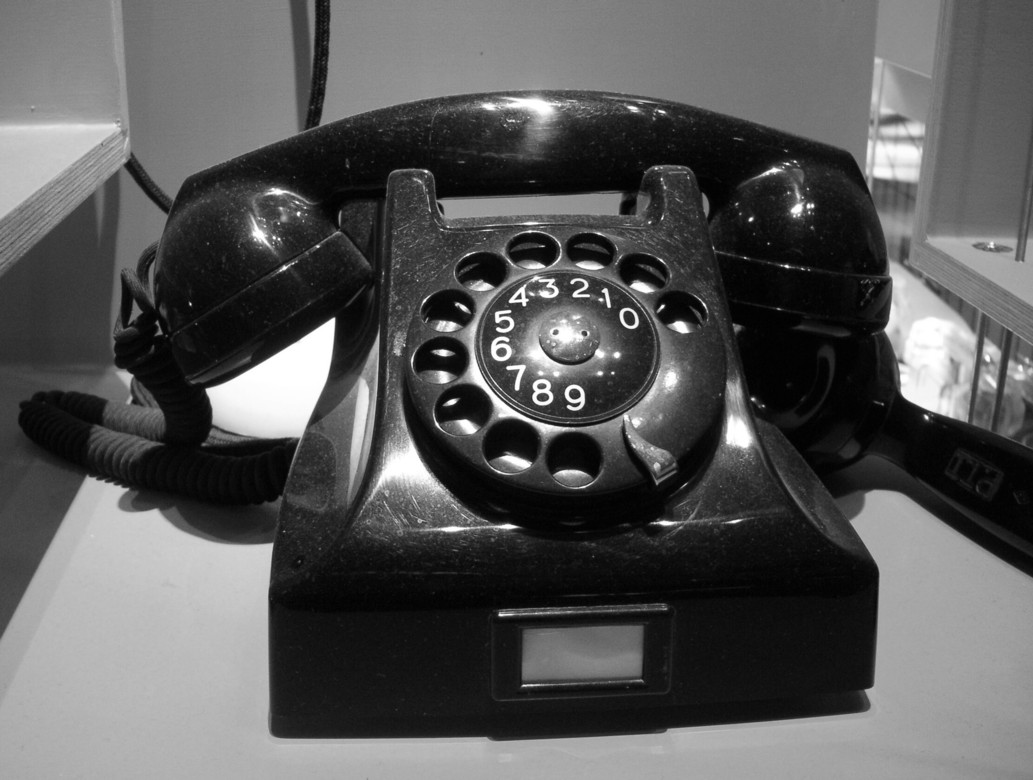
\includegraphics[width=0.42\linewidth]{images/book1/bakelite-telephone.jpg}

{\small 1947 年的电木电话。照片：Holger Ellgaard，
CC BY-SA 3.0。}
\end{omfigure}

\section{主要塑料及其识别码}

\begin{definition}[树脂识别码]\label{def:g8:plastics:code}
\emph{树脂识别码}\index{树脂识别码}是一个 1 至 7 的数字，
印在塑料制品上由箭头组成的三角形内，用来标明
该制品所用的塑料，以便回收时分类。
三角形并不表示该制品
一定会被回收。
\end{definition}

> \begin{proposition}[七种识别码]\label{prop:g8:plastics:codes}
各识别码及其所对应塑料的最常见用途：
\begin{center}
\small
\begin{tabular}{cll}
\hline
识别码 & 塑料 & 典型制品 \\
\hline
1 & PET，聚对苯二甲酸乙二醇酯 & 水瓶和汽水瓶、抓绒纤维 \\
2 & HDPE，高密度聚乙烯 & 牛奶瓶和洗发水瓶、瓶盖 \\
3 & PVC，聚氯乙烯 & 管道、窗框、电缆 \\
4 & LDPE，低密度聚乙烯 & 袋子、薄膜 \\
5 & PP，聚丙烯 & 酸奶杯、瓶盖、汽车保险杠 \\
6 & PS，聚苯乙烯 & 泡沫杯和托盘、CD 盒 \\
7 & 其他塑料 & 混合物、多层包装 \\
\hline
\end{tabular}
\end{center}
\end{proposition}

\begin{omfigure}
\begin{tikzpicture}[font=\small]
  \foreach \n/\lab in {1/PET, 2/HDPE, 3/PVC, 4/LDPE, 5/PP, 6/PS, 7/其他} {
    \begin{scope}[xshift=(\n-1)*2.1cm]
      \foreach \a in {90,210,330} {
        \pgfmathsetmacro\b{\a+120}
        \draw[omDef, line width=1.1pt, ->, >={Stealth[length=4pt]}]
          ($(\a:0.75)!0.14!(\b:0.75)$) -- ($(\a:0.75)!0.86!(\b:0.75)$);
      }
      \node[font=\bfseries] at (0,-0.05) {\n};
      \node[anchor=north, font=\footnotesize] at (0,-0.8) {\lab};
    \end{scope}
  }
\end{tikzpicture}

{\small 七种树脂识别码，每个
标注其塑料的简称。}
\end{omfigure}

\section{热塑性塑料与热固性塑料}

\begin{definition}[热塑性塑料与热固性塑料]\label{def:g8:plastics:thermoplastic}
\emph{热塑性塑料}\index{热塑性塑料}每次加热都会变软，
冷却后又会变硬：可以反复熔化、重新塑形
（PET、聚乙烯、PVC、聚丙烯、聚苯乙烯）。
\emph{热固性塑料}\index{热固性塑料}在首次加热成型后便永久定型：
再次加热时，它不会变软，而是炭化（如电木，
以及胶水和船体所用的树脂）。
\end{definition}

\begin{remark}[哪些可以回收]\label{rem:g8:plastics:which}
热塑性塑料可以熔化后重新塑形，
因此是被回收再制成新制品的塑料。热固性塑料则不能再次熔化。
\end{remark}

\section{环境中的塑料}

\begin{proposition}[塑料难以降解]\label{prop:g8:plastics:last}
% ledger: plastics:use-2019, plastics:waste-2019, plastics:recycled-share-2019
2019 年，全球使用了约 4.6 亿吨塑料，
丢弃了约 3.53 亿吨塑料废弃物；回收塑料
只占所用塑料的约 \qty{6}{\percent}。塑料不会腐烂：
在自然界中，它会碎裂成越来越小的碎片，即微塑料，
在河流、海洋、土壤以及动物体内都能找到它们。
\end{proposition}

\begin{omfigure}
\begin{minipage}[t]{0.48\linewidth}\centering
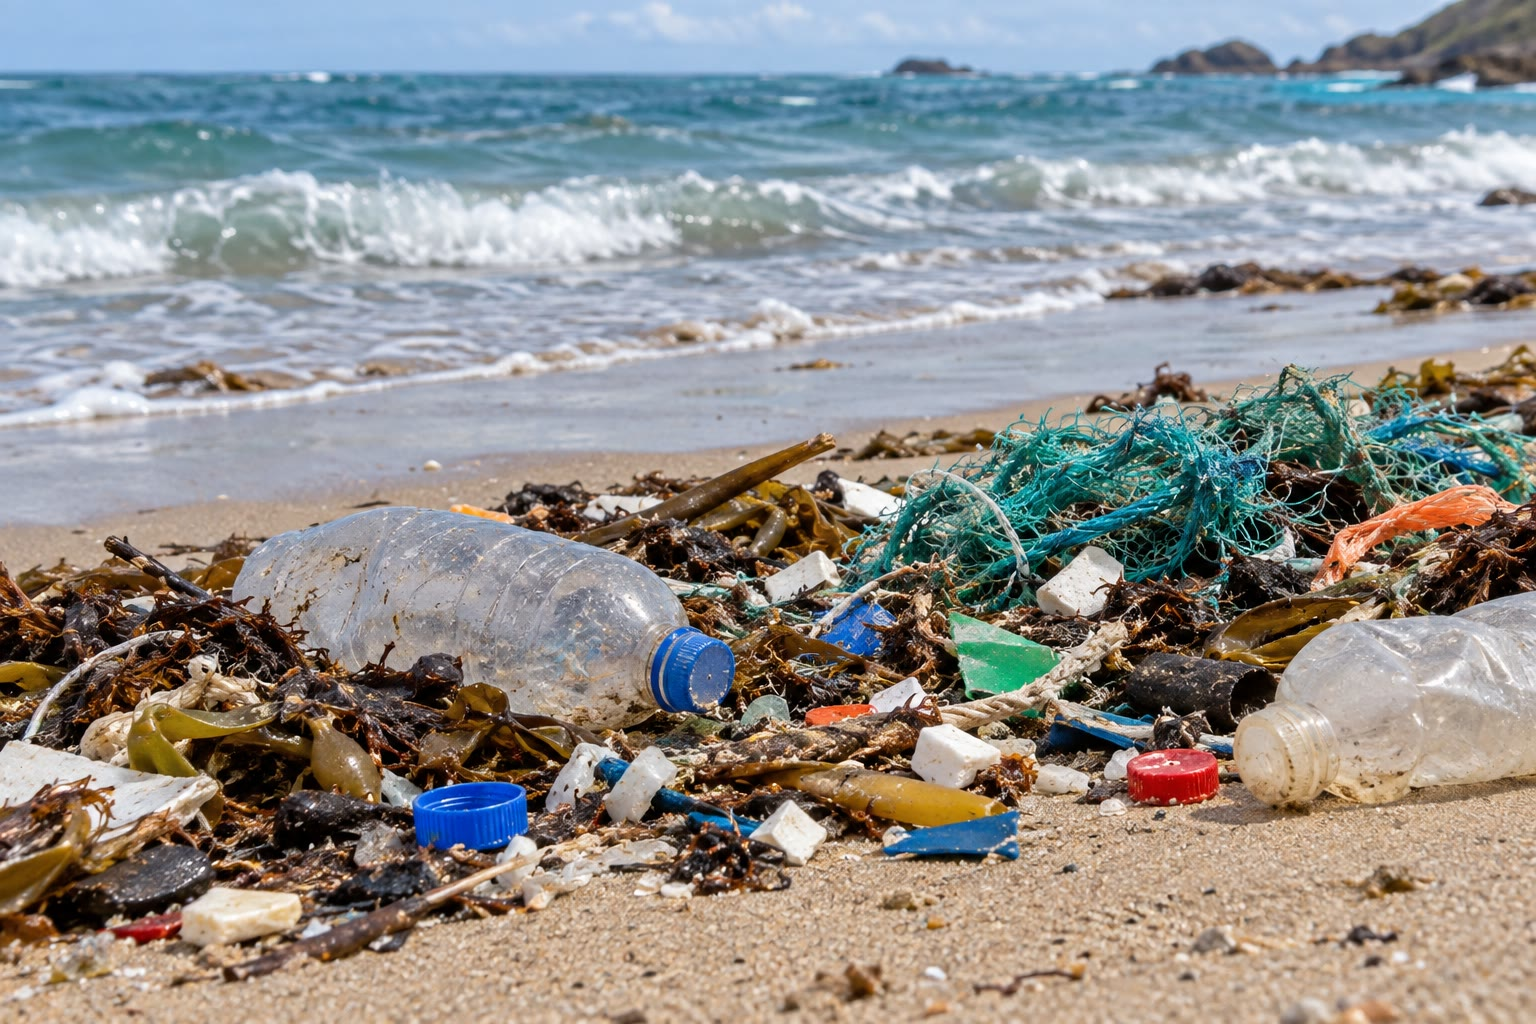
\includegraphics[width=\linewidth,height=4.6cm,keepaspectratio]{images/book1/ai/g8-beach-litter.jpg}

{\small 冲上海滩的塑料垃圾。}
\end{minipage}\hfill
\begin{minipage}[t]{0.48\linewidth}\centering
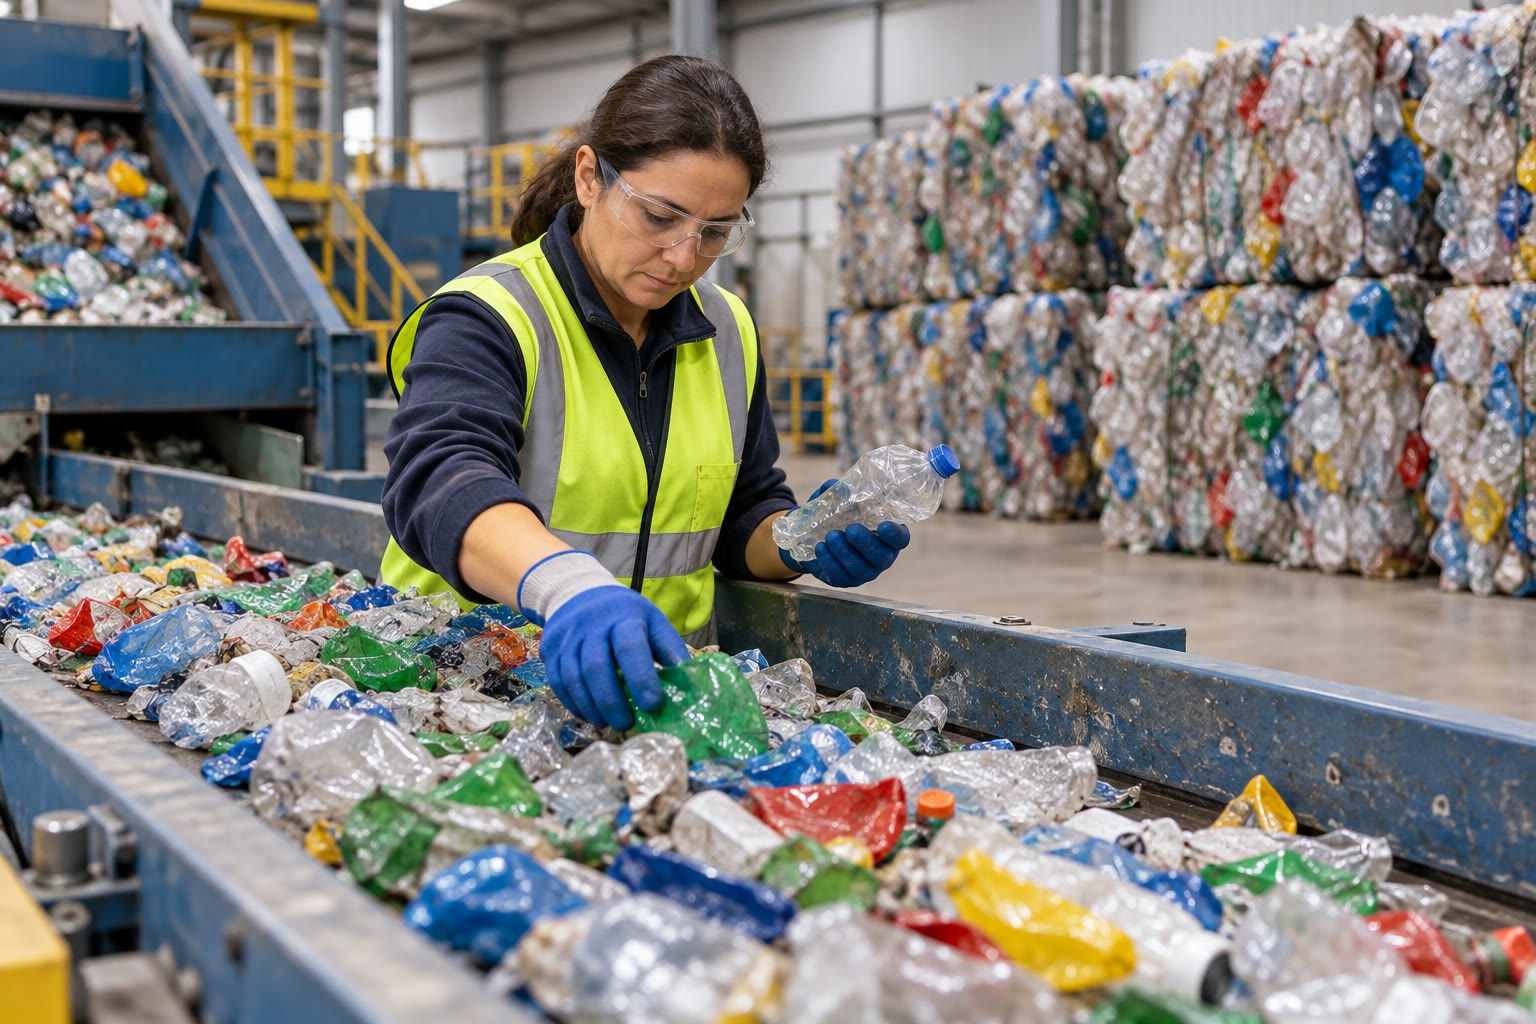
\includegraphics[width=\linewidth,height=4.6cm,keepaspectratio]{images/book1/ai/g8-sorting-line.jpg}

{\small 塑料回收厂中的分拣流水线。}
\end{minipage}
\end{omfigure}

\begin{remark}[燃烧塑料]\label{rem:g8:plastics:burning}
塑料可以燃烧，完全燃烧时会生成二氧化碳。
但在露天火堆中燃烧时，它们是不完全燃烧，会释放出烟炱、
一氧化碳以及其他有害物质；含有氯的 PVC
还会放出氯化氢，这是一种有腐蚀性的气体。塑料废弃物
只能在为净化烟气而建造的焚烧炉中焚烧。
\end{remark}

\section{练习}

\begin{exercise}[$\star$]\label{exo:g8:plastics:1}
天然的、人造的还是合成的？棉、尼龙、纸、羊毛、
聚苯乙烯、黏胶。
\end{exercise}

\begin{exercise}[$\star$]\label{exo:g8:plastics:2}
大多数塑料是由哪种原料制成的？
\end{exercise}

\begin{exercise}[$\star$]\label{exo:g8:plastics:3}
识别码为 1 的是哪种塑料？请举出一种由它制成的制品。
\end{exercise}

\begin{exercise}[$\star$]\label{exo:g8:plastics:4}
热塑性塑料与热固性塑料有什么区别？
\end{exercise}

\begin{exercise}[$\star\star$]\label{exo:g8:plastics:5}
一个酸奶杯上标有识别码 5。请写出它所用的塑料名称，并说明它
原则上能否被熔化后重新塑形。
\end{exercise}

\begin{exercise}[$\star\star$]\label{exo:g8:plastics:6}
为什么物体上画有三角形箭头，并不意味着该物体会
被回收利用？
\end{exercise}

\begin{exercise}[$\star\star$]\label{exo:g8:plastics:7}
为什么煎锅的手柄常由热固性塑料而非
热塑性塑料制成？
\end{exercise}

\begin{exercise}[$\star\star$]\label{exo:g8:plastics:8}
利用本章 2019 年的数据，所用塑料中
有多大百分比在当年成为了废弃物？请四舍五入到最接近的整数。
\end{exercise}

\begin{exercise}[$\star\star$]\label{exo:g8:plastics:9}
为什么绝不能在庭院篝火中焚烧 PVC？
\end{exercise}

\begin{exercise}[$\star\star$]\label{exo:g8:plastics:10}
某学校每周使用 300 个各重 \qty{25}{g} 的瓶子，全年
共使用 36 周。这些塑料一年的质量是多少？
\end{exercise}

\begin{exercise}[$\star\star\star$]\label{exo:g8:plastics:11}
聚乙烯仅由碳和氢组成。写出
其完全燃烧的生成物。说明为何燃烧它会像化石燃料一样向
空气中增加二氧化碳。
\end{exercise}

\begin{exercise}[$\star\star\star$]\label{exo:g8:plastics:12}
说明一只遗落在海上的塑料瓶如何
在数年后变成鱼体内的微塑料。
\end{exercise}

\section{问题：分拣线}

\begin{problem}[{周末问题——一吨旧瓶子、它们的
识别码，以及工厂产出的干净塑料碎片}]
\label{pb:g8:plastics:1}
回收工厂收到一批旧饮料瓶压包。典型的
一包 \qty{1}{t}（\qty{1000}{kg}）按质量计，其中 \qty{80}{\percent} 为
PET 瓶身，\qty{12}{\percent} 为瓶盖（HDPE 和 PP），
\qty{5}{\percent} 为标签（PP 薄膜），\qty{3}{\percent} 为污垢和
残留液体。机器将瓶盖和标签与瓶身分开，
PET 被粉碎成碎片，碎片经清洗；清洗
损失 \qty{2.5}{\percent} 的 PET。干净的碎片被熔化并
纺成抓绒外套的纤维。

\medskip
\noindent\textbf{第一部分——塑料。}
\begin{enumerate}
  \item 瓶身上印有哪个识别码？瓶盖上呢？
  \item 这些塑料是天然的、人造的还是合成的？
  \item PET 能否再次熔化并纺丝？这说明它属于
        哪一类塑料？
  \item 为什么要在 PET 熔化之前，先把瓶盖和标签
        与瓶身分开？
\end{enumerate}

\medskip
\noindent\textbf{第二部分——压包。}
\begin{enumerate}[resume]
  \item 一包压包中含有多少质量的 PET？
  \item 瓶盖的质量是多少？标签呢？
  \item 压包中非塑料部分的质量是多少？
  \item 压包中塑料所占的百分比是多少？
\end{enumerate}

\medskip
\noindent\textbf{第三部分——碎片。}
\begin{enumerate}[resume]
  \item 清洗过程中损失了多少质量的 PET？
  \item 一件抓绒外套需要 \qty{0.39}{kg} 的 PET 纤维，为什么
        用碎片制造比用新 PET 更好？
  \item 工厂本可以燃烧瓶盖和标签来取热，而不是
        回收它们。请写出这一做法会向空气中添加的气体名称。
  \item 计算一包压包所产出的干净 PET 碎片的质量。
\end{enumerate}
\end{problem}
